\documentclass[11pt,letter]{article}
\usepackage[top=0.30in, bottom=0.7in, left=1.1in, right=1.1in]{geometry}
\usepackage{graphicx} % Required for inserting images
\usepackage{xcolor} 
\usepackage{amsmath}
\usepackage{gensymb}
\definecolor{Accent}{HTML}{bd2b00} 
\usepackage{natbib}
\usepackage{hyperref}
\hypersetup{colorlinks,citecolor = Accent, linkcolor = Accent,urlcolor = Accent, breaklinks=true}
\usepackage{cleveref}
\usepackage[labelfont=bf]{caption}
\bibliographystyle{amnat}

\RequirePackage[labelfont={bf,sf},%
                font={small, sf}]{caption}


\let\oldthefigure\thefigure
\renewcommand{\thefigure}{S\oldthefigure}

\title{Solstice optimizes thermal growing season\\\emph{Supplementary materials}}

\author{Victor, Lizzie}
\date{Aug.-Dec. 2024}

\begin{document}

\maketitle

\section*{Supplementary methods} %emw19Jan -- this supplement is really amazing! If we don't end up in a short-form journal, I will. be very happy to see much of this in a main text somewhere!

%emw19Jan -- I would use active voice a little more, but this sees okay. 
All analyses were run on \textbf{\textsf{R}}, using the package \texttt{terra} for raster manipulation \citep{Hijmans2024}. The workflow of the analysis is represented in the \Cref{fig:method}.

\paragraph{Climate data}
Daily mean temperatures from 1951 to 2020 were extracted from the ERA5-Land dataset, at a 0.1\degree~spatial resolution \citep{MunozSabater2021}. We sampled $>$500 sites on a regular grid across Europe (see Figure 2 in the main text).\\
Following \citet{McMaster1997}, we define growing degree-days at a day d ($GDD_d$) as:
\begin{equation}
GDD_d =
\begin{cases}
    0 & \text{if}~T_d<T_{lower}\\
    T_{upper}-T_{lower} & \text{if}~T_d>T_{upper}\\
    T_d-T_{lower} & \text{otherwise}
\end{cases}       
\end{equation}

\noindent where $T_d$ is the mean temperature at the day $d$, and $T_{lower}$/$T_{upper}$ the lower/upper temperature thresholds (defining the range within which metabolism is likely active). Here, we chose $T_{lower}=5$\degree C and $T_{upper}=35$\degree C (see \Cref{fig:altgdd} for the same analysis with 0-40\degree C range). 

\paragraph{Optimal period} For each day and each site, environmental predictability was computed as the $R^2$ of the linear regression across years between total GDD and the GDD accumulated by that day (blue panel, \Cref{fig:method}). Growth potential was defined as the remaining GDD to be accumulated from that day until the end of the year (yellow panel, \Cref{fig:method}). While other trade-offs could be considered, we chose this as the simplest option (and perhaps most obvious), especially given our limited understanding of the underlying loss functions plants may rely on. Both environmental predictability and growth potential were computed for the entire year (January 1 to December 31), although the growing season is likely more restricted and varies across locations. \\
%emw19Jan -- Can you explain where the 1.414 comes from a little? 
We computed an optimality measure based on the Euclidean distance $D$ from  the ideal point where both predictability and growth potential (scaled to $[0,1]$) are maximized (green panel, \Cref{fig:method}). Optimality was defined as $max(D)-D$ (where $max(D)\approx1.414$)---such that higher values correspond to more optimal days. Days were classified as optimal if they fell within the top 10\% of days with the higher optimality.

\begin{figure}[hb]
\hspace*{-1.4cm}
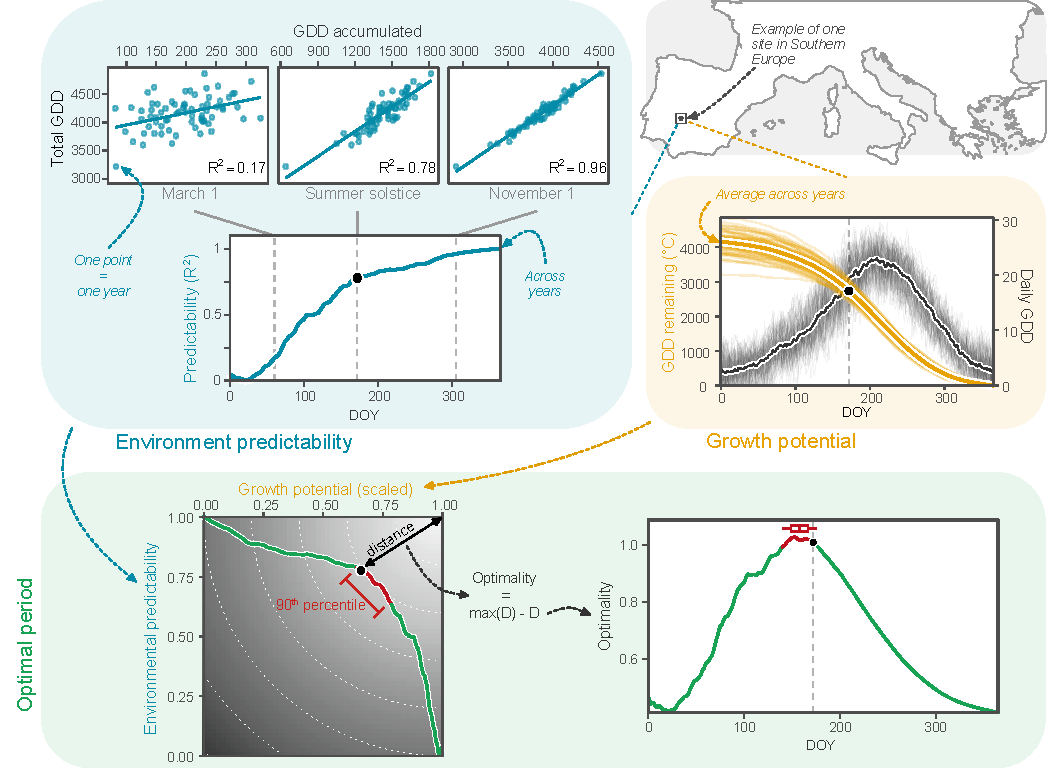
\includegraphics{method_figure.pdf}
\vspace*{-0.4cm}
\caption{\textbf{Workflow of the optimality analysis for one site in Southern Europe.}} %emw19Jan -- This figure is so nice and super helpful for readers.
\label{fig:method}
\end{figure}

\clearpage

\begin{figure}[h]
\centering
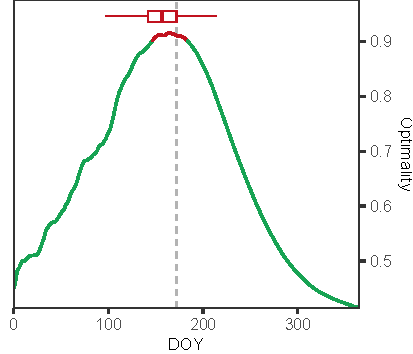
\includegraphics{global_optimality_0_40.pdf} %emw19Jan -- I would contrast this a bit more with the next figure in the caption similar to what I suggested in main text. So in the next figure caption you should stress how this is different from findings of the average and here you could even reference the next figure if you like.... 
\vspace*{-0.4cm}
\caption{\textbf{Average optimal trade-off between environmental predictability and growth potential across Europe, with an alternative GDD definition} ($T_{lower}=0$\degree C and $T_{upper}=40$\degree C).}
\label{fig:altgdd}
\end{figure}


\begin{figure}[h]
\hspace*{-1.2cm}
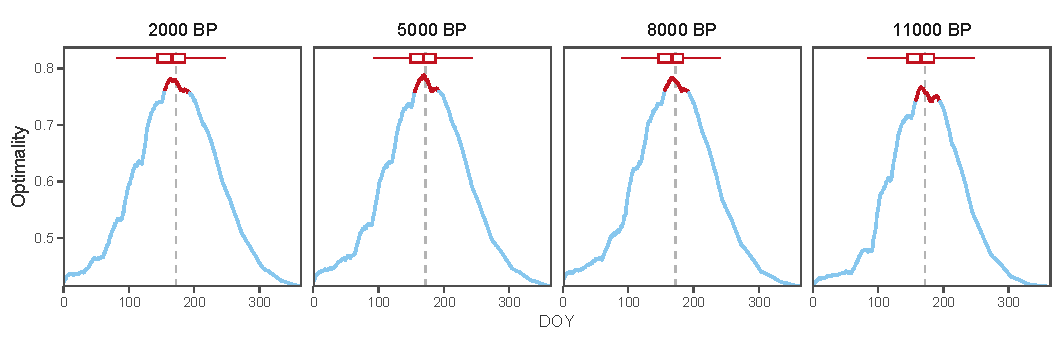
\includegraphics[scale = 1]{optimality_holocene.pdf}
\vspace*{-0.7cm}
\caption{\textbf{The average optimal trade-off between environmental predictability and growth potential is relatively stable across the Holocene.} Daily mean temperatures were obtained from \citet{VanderMeersch2024}, in which daily data were generated with the GWGEN weather generator \citep{Sommer2017} based on monthly paleosimulations from the HadCM3B-M2.1 coupled general circulation model \citep{Armstrong2019}. BP stand for "Before Present" (i.e. 1950).}
\label{fig:holocene}
\end{figure}


\vspace*{-0.7cm}
\begin{figure}[h]
\centering
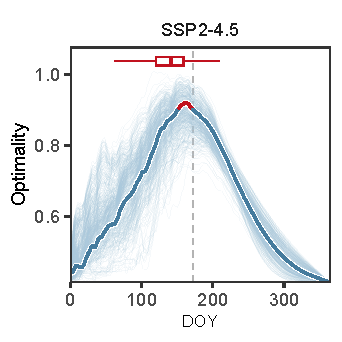
\includegraphics{optimality_future.pdf}
\vspace*{-0.5cm}
\caption{\textbf{Average optimal trade-off between environmental predictability and growth potential in future climates (2071-2100).} Daily mean temperatures came from the last Coupled Model Intercomparison Project Phase 6 (CMIP6) climate  projections, for 5 global climate models (GCMs) and 2 shared socio-economic pathways (SSPs). Model projections were downscaled to a 0.1° resolution with a statistical trend-preserving method (the cumulative distribution function transform), using the ERA5-Land reanalysis as a reference observational dataset between 1981 and 2010 \citep{Noel2022}. Thin lines represent the five GCMs (GFDL-ESM4, IPSL-CM6A-LR, MPI-ESM1-2-HR, MRI-ESM2-0 and UKESM1-0-LL), large lines represent the average across GCMs.}
\label{fig:future}
\vspace*{-10cm}
\end{figure}

\clearpage

\vspace*{-1.2cm}
\begin{figure}[h]
\centering
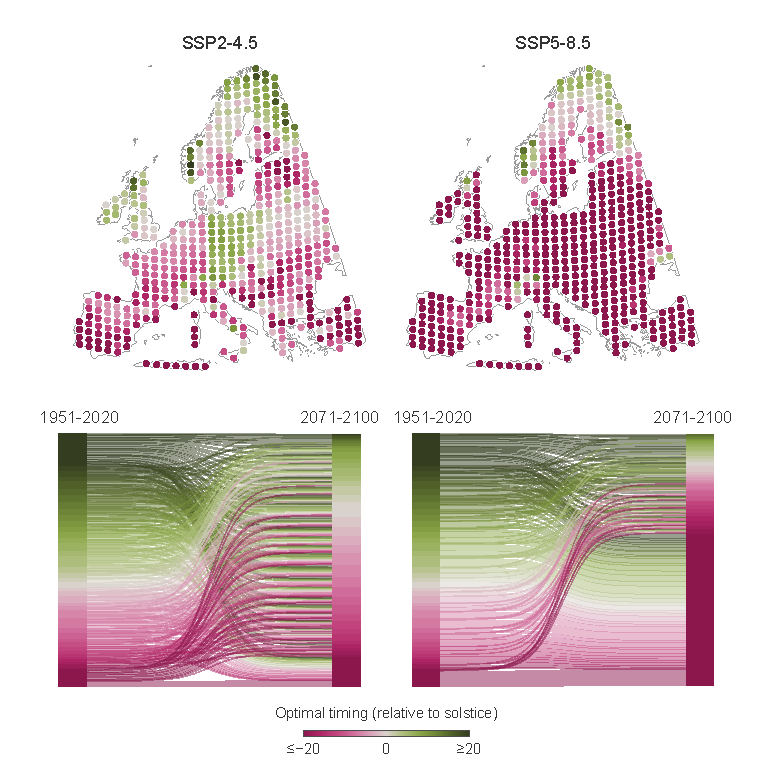
\includegraphics[scale = 1]{local_optimality_future.pdf}
\vspace*{-0.4cm}
\caption{\textbf{Solstice may not represent a reliable cue to track the optimal period under future climatic conditions (2071-2100).} On the top panel, sites are sampled on a regular grid across Europe. On the bottom panel, Sankey diagrams show the proportional flow of (site-specific) optimal timing from 1951-2020 to 2071-2100. Colors indicate the timing—relative to the solstice—of the median optimal day.}
\label{fig:holocene}
\end{figure}

{\footnotesize
\vspace*{0cm}
\bibliography{synchrony}}

\end{document}
